\section{Satz von Pythagoras, Länge und Skalarprodukt}
		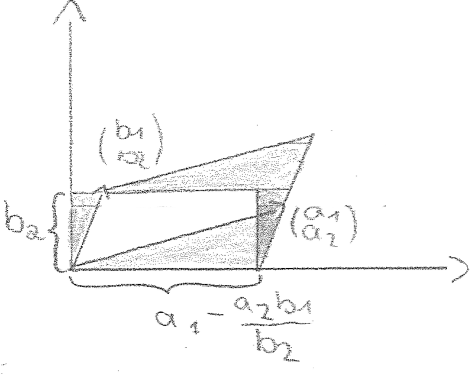
\includegraphics[width=0.35\textwidth]
	{mainmatter/chapter1/pics/parallelogram.png}Fläche des Parallelogramms gleich $|det(\vec{a},\vec{b})|$\\
$\begin{pmatrix} a_{1} \\ a_{2} \end{pmatrix} + \lambda \begin{pmatrix} b_{1} \\ b_{2} \end{pmatrix} = \begin{pmatrix} x \\ 0 \end{pmatrix} \mathop{\Rightarrow}\limits^{b_{2} \neq 0} \lambda = \frac{-a_{2}}{b_{2}}, x=a_{1}-\frac{a_{2}b_{1}}{b_{2}}$ \\
Rechteck hat Fläche $\vert a_{1}b_{2}-a_{2}b_{1}\vert=\vert det(a,b) \vert =$ Fläche des Parallelogramms. 
%
%
%
\subsection{Satz des Pythagoras (1. Version)}
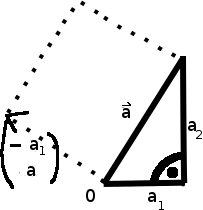
\includegraphics[width=0.15\textwidth]
	{mainmatter/chapter1/pics/pyth.png}$\vec{a} = \begin{pmatrix} a_{1} \\ a_{2} \end{pmatrix}$ hat Länge $\Vert \vec{a} \Vert = \sqrt{a_{1}^{2} + a_{2}^{2}}$
%
%
%
\subsubsection{Beweis:}
$det(\vec{a},\vec{a}_{\perp})=a_{1}^{2+}a_{2}^{2}$ ist das Quadrat der Seitenlänge $\sqrt{a_{1}^{2}+a_{2}^{2}}$
%
%
%
\subsubsection{Definition:}
Der Abstand zweier Vektoren $\vec{a}$ und $\vec{b}$ ist $ \qquad \Vert \vec{a}-\vec{b} \Vert$
%
%
%
\subsubsection{Bemerkung:}
$\begin{pmatrix} a_{1} \\ a_{2} \end{pmatrix} \perp \begin{pmatrix} b_{1} \\ b_{2} \end{pmatrix} \Rightarrow \begin{pmatrix} b_{1} \\ b_{2} \end{pmatrix} = \lambda \begin{pmatrix} -a_{2} \\ a_{1} \end{pmatrix} \Leftrightarrow a_{1}b_{1}+a_{2}b_{2}=0$
\begin{description}
	\item["`$\Rightarrow$"'] $a_{1}b_{1}+a_{2}b_{2}= -\lambda a_{1}a_{2} + \lambda 
		a_{1}a_{2}$
	\item["`$\Leftarrow$"'] Falls $ a = \begin{pmatrix} 0 \\ 0 \end{pmatrix} \leadsto 
		\lambda = 0$ \\ 
		o.E. $a_{1} \neq 0 $ \\
		setze $\lambda: b_{2} = \lambda a_{1} \mathop{\Rightarrow}\limits^{\text{Vor.}} 
		0 = a_{1}b_{1}+ a_{1}\cdot\lambda a_{1}a_{2} \Rightarrow b_{1} = - 
		\lambda a_{2}$
\end{description}
%
%
%
\subsubsection{Definition:}
Skalarprodukt\\
Das von $\vec{a}$ und $\vec{b}: <\vec{a},\vec{b}> = a_{1}b_{1}+a_{2}b_{2}$.
%
%
%
\subsubsection{Eigenschaften des Skalarprodukts}
$<\vec{a}+\vec{b},\vec{c}>=(a_{1}+b_{1})c_{1}+(a_{2}+b_{2})c_{2}=<a,c>+<b,c>$\\
$<\lambda \vec{a},\vec{b}>=\lambda <\vec{a},\vec{b}>$\\
$<\vec{a},\vec{b}>=<\vec{b},\vec{a}>$
%
%
%
\subsection{Pythagoras (allgemein)}
$\vec{a}\perp\vec{b} \Rightarrow \Vert \vec{a} - \vec{b} \Vert^{2} = \Vert \vec{a} \Vert^{2} + \Vert \vec{b} \Vert ^{2}$
%
%
%
\subsubsection{Beweis:}
$<\vec{a},\vec{b}>=0 $\\
$\Vert \vec{a} - \vec{b} \Vert^{2} = (a_{1}-b_{1})^{2} + (a_{2} - b_{2})^{2} = a_{1}^{2}+b_{1}^{2}+a_{2}^{2}+b_{2}^{2} = \Vert \vec{a} \Vert^{2} + \Vert \vec{b} \Vert^{2}$
%
%
%
\subsection{Satz des Thales}
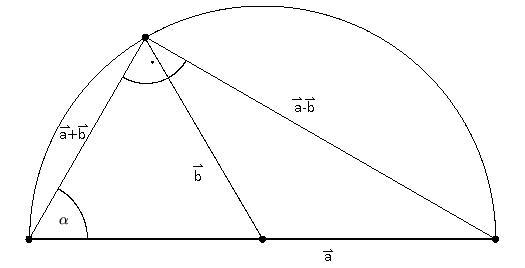
\includegraphics[width=0.5\textwidth]
	{mainmatter/chapter1/pics/satzdesthales.png}\\
	
$\vec{a},\vec{b}: \Vert \vec{a} \Vert =\Vert \vec{b} \Vert \Rightarrow \vec{a} - \vec{b} \perp  \vec{a} + \vec{b}$
%
%
%
\subsubsection{Beweis:}
$<\vec{a}-\vec{b},\vec{a} + \vec{b}> = <\vec{a},\vec{b}>-<\vec{b},\vec{a}>+<\vec{a},\vec{a}>-<\vec{b},\vec{b}>=0$
%
%
%
\subsubsection{Satz:}
Sei $l$ Gerade, $c \notin l$. \\
Dann existiert genau ein "`Fußpunkt"' $D \in l: c-D\perp l$
%
%
%
\subsubsection{Beweis:}
$\vec{n} \perp l$. Schneide $c+ \mathbb{R}\vec{n}$  mit $l$. \\
$det(\vec{n},\vec{n}^{\perp})=\Vert \vec{n}\Vert^{2} \neq 0 \Rightarrow$ es existiert $D$ 
%
%
%
\subsubsection{Höhensatz}
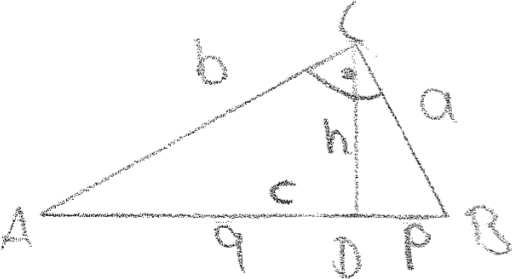
\includegraphics[width=0.3\textwidth]
	{mainmatter/chapter1/pics/heohensatz.png}\\
	$ABC$ sei ein rechtwinkliges Dreieck
	$p=\Vert D-B \Vert \qquad q=\Vert D-A\Vert \qquad h=\Vert D-C\Vert \Rightarrow h^{2}=pq$
%
%
%
\subsubsection{Beweis:}
$a^{2} + b^{2} = c^{2} = p^{2} + 2pq + q^{2}$\\
$a^{2}=h^{2}+p^{2}$\\
$b^{2}=h^{2}+q^{2}$\\
\qquad\\
$\Rightarrow p^{2} + 2pq +q^{2} = 2h^{2}+p^{2}+q^{2}$\\
$\Leftrightarrow 2pq = 2h^{2}$\\
$\Leftrightarrow pq=h^{2} \qquad \square$
%
%
%
\subsubsection{Kathetensatz}
$ABC$ sei ein rechtwinkliges Dreieck
$a^{2} = p\cdot c, b^{2} = q\cdot c$
%
%
%
\subsubsection{Beweis:}
$a^{2} = c^{2}-b^{2}=p^{2}+2pq+q^{2}-(h^{2}+q^{2})=p^{2}+2pq-h^{2}=p^{2}+2pq-a^{2}+p^{2}$\\
\qquad\\
$2a^{2}=2pq+2p^{2}$\\
$\Leftrightarrow a^{2} = pq+p^{2} \Rightarrow$ Behauptung; analog für $b^{2} = qc \qquad\square$